% Arquivo LaTeX de exemplo de monografia para a disciplina MAC0499
%
% Adaptado em julho/2015 a partir do
%
% ---------------------------------------------------------------------------- %
% Arquivo LaTeX de exemplo de dissertação/tese a ser apresentados à CPG do IME-USP
%
% Versão 5: Sex Mar  9 18:05:40 BRT 2012
%
% Criação: Jesús P. Mena-Chalco
% Revisão: Fabio Kon e Paulo Feofiloff


\documentclass[12pt,twoside,a4paper]{book}


% ---------------------------------------------------------------------------- %
% Pacotes
\usepackage[utf8]{inputenc}
\usepackage[T1]{fontenc}
\usepackage[brazil]{babel}
\usepackage[pdftex]{graphicx}           % usamos arquivos pdf/png como figuras
\usepackage{setspace}                   % espaçamento flexível
\usepackage{indentfirst}                % indentação do primeiro parágrafo
\usepackage{makeidx}                    % índice remissivo
\usepackage[nottoc]{tocbibind}          % acrescentamos a bibliografia/indice/conteudo no Table of Contents
\usepackage{courier}                    % usa o Adobe Courier no lugar de Computer Modern Typewriter
\usepackage{type1cm}                    % fontes realmente escaláveis
\usepackage{listings}                   % para formatar código-fonte (ex. em Java)
\usepackage{titletoc}
%\usepackage[bf,small,compact]{titlesec} % cabeçalhos dos títulos: menores e compactos
\usepackage[fixlanguage]{babelbib}
\usepackage[font=small,format=plain,labelfont=bf,up,textfont=it,up]{caption}
\usepackage[usenames,svgnames,dvipsnames]{xcolor}
\usepackage[a4paper,top=2.54cm,bottom=2.0cm,left=2.0cm,right=2.54cm]{geometry} % margens
%\usepackage[pdftex,plainpages=false,pdfpagelabels,pagebackref,colorlinks=true,citecolor=black,linkcolor=black,urlcolor=black,filecolor=black,bookmarksopen=true]{hyperref} % links em preto
\usepackage[pdftex,plainpages=false,pdfpagelabels,pagebackref,colorlinks=true,citecolor=DarkGreen,linkcolor=NavyBlue,urlcolor=DarkRed,filecolor=green,bookmarksopen=true]{hyperref} % links coloridos
\usepackage[all]{hypcap}                    % soluciona o problema com o hyperref e capitulos
\usepackage[round,sort,nonamebreak]{natbib} % citação bibliográfica textual(plainnat-ime.bst)
\usepackage{emptypage}  % para não colocar número de página em página vazia
\fontsize{60}{62}\usefont{OT1}{cmr}{m}{n}{\selectfont}

% ---------------------------------------------------------------------------- %
% Cabeçalhos similares ao TAOCP de Donald E. Knuth
\usepackage{fancyhdr}
\pagestyle{fancy}
\fancyhf{}
\renewcommand{\chaptermark}[1]{\markboth{\MakeUppercase{#1}}{}}
\renewcommand{\sectionmark}[1]{\markright{\MakeUppercase{#1}}{}}
\renewcommand{\headrulewidth}{0pt}

% ---------------------------------------------------------------------------- %
\graphicspath{{./figuras/}}             % caminho das figuras (recomendável)
\frenchspacing                          % arruma o espaço: id est (i.e.) e exempli gratia (e.g.)
\urlstyle{same}                         % URL com o mesmo estilo do texto e não mono-spaced
\makeindex                              % para o índice remissivo
\raggedbottom                           % para não permitir espaços extra no texto
\fontsize{60}{62}\usefont{OT1}{cmr}{m}{n}{\selectfont}
\cleardoublepage
\normalsize

% ---------------------------------------------------------------------------- %
% Opções de listing usados para o código fonte
% Ref: http://en.wikibooks.org/wiki/LaTeX/Packages/Listings
\lstset{ %
language=Java,                  % choose the language of the code
basicstyle=\footnotesize,       % the size of the fonts that are used for the code
numbers=left,                   % where to put the line-numbers
numberstyle=\footnotesize,      % the size of the fonts that are used for the line-numbers
stepnumber=1,                   % the step between two line-numbers. If it's 1 each line will be numbered
numbersep=5pt,                  % how far the line-numbers are from the code
showspaces=false,               % show spaces adding particular underscores
showstringspaces=false,         % underline spaces within strings
showtabs=false,                 % show tabs within strings adding particular underscores
frame=single,	                % adds a frame around the code
framerule=0.6pt,
tabsize=2,	                    % sets default tabsize to 2 spaces
captionpos=b,                   % sets the caption-position to bottom
breaklines=true,                % sets automatic line breaking
breakatwhitespace=false,        % sets if automatic breaks should only happen at whitespace
escapeinside={\%*}{*)},         % if you want to add a comment within your code
backgroundcolor=\color[rgb]{1.0,1.0,1.0}, % choose the background color.
rulecolor=\color[rgb]{0.8,0.8,0.8},
extendedchars=true,
xleftmargin=10pt,
xrightmargin=10pt,
framexleftmargin=10pt,
framexrightmargin=10pt
}

% ---------------------------------------------------------------------------- %
% Corpo do texto
\begin{document}

\frontmatter
% cabeçalho para as páginas das seções anteriores ao capítulo 1 (frontmatter)
\fancyhead[RO]{{\footnotesize\rightmark}\hspace{2em}\thepage}
\setcounter{tocdepth}{2}
\fancyhead[LE]{\thepage\hspace{2em}\footnotesize{\leftmark}}
\fancyhead[RE,LO]{}
\fancyhead[RO]{{\footnotesize\rightmark}\hspace{2em}\thepage}

\onehalfspacing  % espaçamento

% ---------------------------------------------------------------------------- %
% CAPA
\thispagestyle{empty}
\begin{center}
    \vspace*{2.3cm}
    Universidade de São Paulo\\
    Instituto de Matemática e Estatística\\
    Bachalerado em Ciência da Computação


    \vspace*{3cm}
    \Large{Nome completo do Autor}


    \vspace{3cm}
    \textbf{\Large{Título da monografia \\
    se for longo ocupa esta linha também}}


    \vskip 5cm
    \normalsize{São Paulo}

    \normalsize{Dezembro de 2015}
\end{center}

% ---------------------------------------------------------------------------- %
% Página de rosto
%
\newpage
\thispagestyle{empty}
    \begin{center}
        \vspace*{2.3 cm}
        \textbf{\Large{Título da monografia \\
    se for longo ocupa esta linha também}}
        \vspace*{2 cm}
    \end{center}

    \vskip 2cm

    \begin{flushright}
	Monografia final da disciplina \\
        MAC0499 -- Trabalho de Formatura Supervisionado.
    \end{flushright}

    \vskip 5cm

    \begin{center}
    Supervisor: Prof. Dr. Nome do Supervisor\\
    $[$ Cosupervisor: Prof. Dr. Nome do Cosupervisor $]$

    \vskip 5cm
    \normalsize{São Paulo}

    \normalsize{Dezembro de 2015}
    \end{center}
\pagebreak




\pagenumbering{roman}     % começamos a numerar

%% % ---------------------------------------------------------------------------- %
%% % Agradecimentos:
%% % Se o candidato não quer fazer agradecimentos, deve simplesmente eliminar esta página
%% \chapter*{Agradecimentos}
%% Texto texto texto texto texto texto texto texto texto texto texto texto texto
%% texto texto texto texto texto texto texto texto texto texto texto texto texto
%% texto texto texto texto texto texto texto texto texto texto texto texto texto
%% texto texto texto texto. Texto opcional.



% ---------------------------------------------------------------------------- %
% Resumo
\chapter*{Resumo}

Elemento obrigatório, constituído de uma sequência de frases concisas e
objetivas, em forma de texto.  Deve apresentar os objetivos, métodos empregados,
resultados e conclusões.  O resumo deve ser redigido em parágrafo único, conter
no máximo 500 palavras e ser seguido dos termos representativos do conteúdo do
trabalho (palavras-chave).
\\

\noindent \textbf{Palavras-chave:} palavra-chave1, palavra-chave2, palavra-chave3.

% ---------------------------------------------------------------------------- %
% Abstract
\chapter*{Abstract}

Elemento obrigatório, elaborado com as mesmas características do resumo em
língua portuguesa.
\\

\noindent \textbf{Keywords:} keyword1, keyword2, keyword3.


% ---------------------------------------------------------------------------- %
% Sumário
\tableofcontents    % imprime o sumário




%% % ---------------------------------------------------------------------------- %
%% \chapter{Lista de Abreviaturas}
%% \begin{tabular}{ll}
%%          CFT         & Transformada contínua de Fourier (\emph{Continuous Fourier Transform})\\
%%          DFT         & Transformada discreta de Fourier (\emph{Discrete Fourier Transform})\\
%%         EIIP         & Potencial de interação elétron-íon (\emph{Electron-Ion Interaction Potentials})\\
%%         STFT         & Tranformada de Fourier de tempo reduzido (\emph{Short-Time Fourier Transform})\\
%% \end{tabular}

%% % ---------------------------------------------------------------------------- %
%% \chapter{Lista de Símbolos}
%% \begin{tabular}{ll}
%%         $\omega$    & Frequência angular\\
%%         $\psi$      & Função de análise \emph{wavelet}\\
%%         $\Psi$      & Transformada de Fourier de $\psi$\\
%% \end{tabular}

%% % ---------------------------------------------------------------------------- %
%% % Listas de figuras e tabelas criadas automaticamente
%% \listoffigures
%% \listoftables



% ---------------------------------------------------------------------------- %
% Capítulos do trabalho
\mainmatter

% cabeçalho para as páginas de todos os capítulos
\fancyhead[RE,LO]{\thesection}

\singlespacing              % espaçamento simples
%\onehalfspacing            % espaçamento um e meio


\input cap-introducao        % associado ao arquivo: 'cap-introducao.tex'
\input cap-desenvolvimentos  % associado ao arquivo: 'cap-desenvolvimento.tex'
\input cap-conclusoes        % associado ao arquivo: 'cap-conclusoes.tex'

% cabeçalho para os apêndices
\renewcommand{\chaptermark}[1]{\markboth{\MakeUppercase{\appendixname\ \thechapter}} {\MakeUppercase{#1}} }
\fancyhead[RE,LO]{}
\appendix

\chapter{grafo completo grmonty CUDA}
\label{cap:ape}

\begin{sidewaysfigure}[!h]
  \centering
  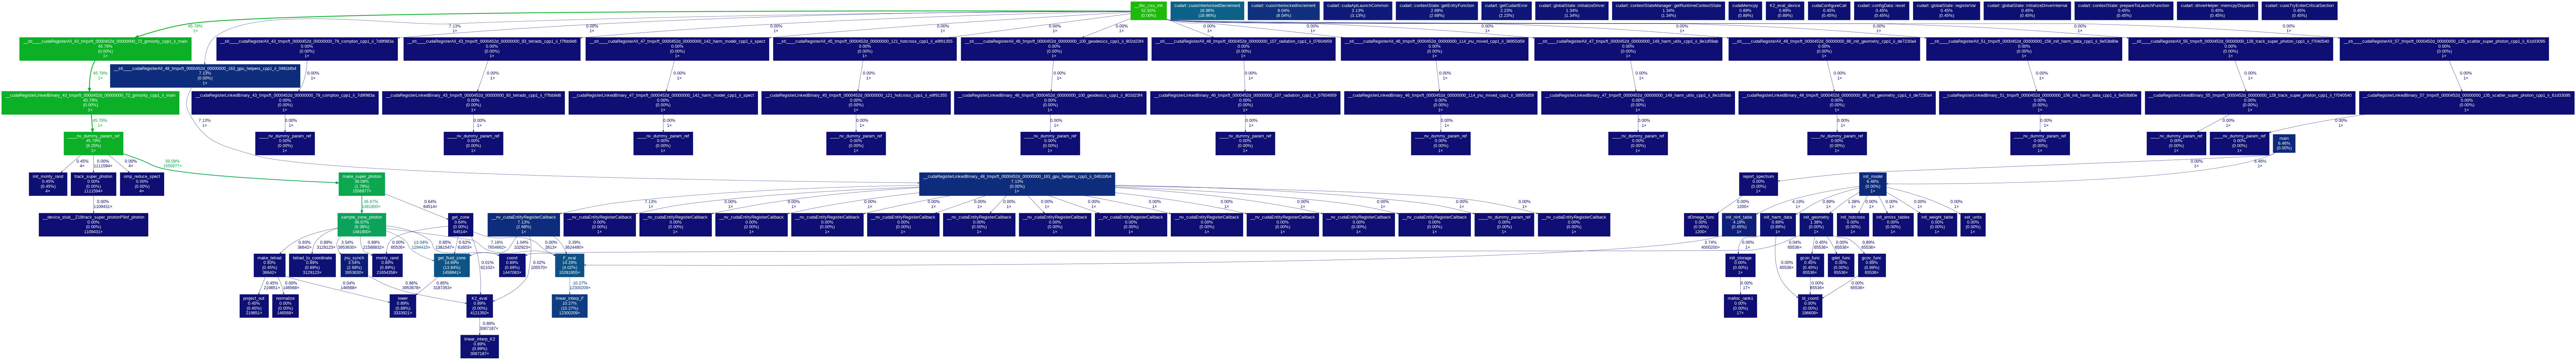
\includegraphics[height=0.106\textwidth]{fullcuda.png}
  \caption{grafo completo com todas as chamadas e com seus respectivos usos. código ja em CUDA. Porcentagens iguais a zero não indicam que o program não execuou essas chamdas e sim que que o g prof não foi capaz de medir o tempo gasto nelas}
  \label{fig:fullcuda}
\end{sidewaysfigure}
      % associado ao arquivo: 'ape-conjuntos.tex'


% ---------------------------------------------------------------------------- %
% Bibliografia
\backmatter \singlespacing   % espaçamento simples
\bibliographystyle{plainnat-ime} % citação bibliográfica textual
\bibliography{bibliografia}  % associado ao arquivo: 'bibliografia.bib'


%%%  ---------------------------------------------------------------------------- %
%% % Índice remissivo
%% \index{TBP|see{periodicidade região codificante}}
%% \index{DSP|see{processamento digital de sinais}}
%% \index{STFT|see{transformada de Fourier de tempo reduzido}}
%% \index{DFT|see{transformada discreta de Fourier}}
%% \index{Fourier!transformada|see{transformada de Fourier}}

%% \printindex   % imprime o índice remissivo no documento

\end{document}
